\documentclass[border=4pt]{standalone}

\usepackage[T1]{fontenc}
\usepackage[utf8]{inputenc}
\usepackage{amsmath}
\usepackage{xcolor}
\usepackage{tikz}
\usetikzlibrary{arrows.meta}

\begin{document}

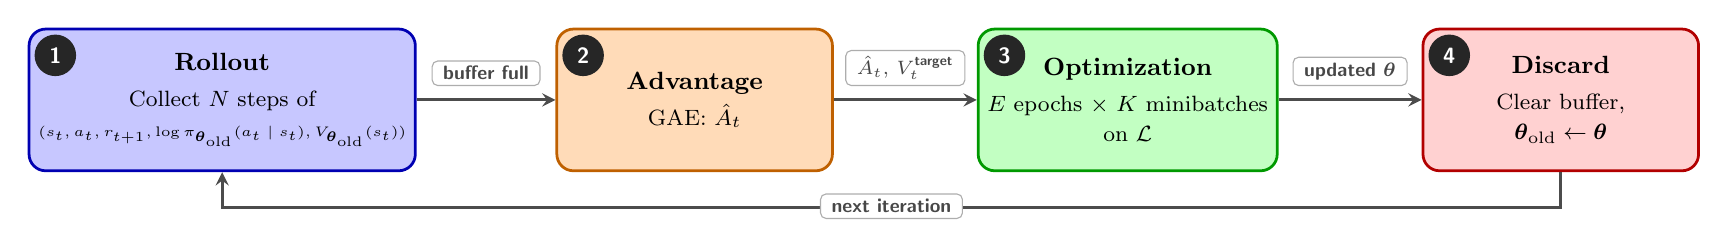
\begin{tikzpicture}[
    every node/.style={transform shape},
    stepbox/.style={
        draw, line width=1pt, rounded corners=6pt,
        minimum width=3.5cm, minimum height=1.8cm,
        align=center, font=\small\bfseries
    },
    arrow/.style={-stealth, line width=1.1pt, black!70},
    % soft arrow labels (white chip, thin gray border) ──
    lbl/.style={font=\scriptsize\bfseries\sffamily, text=black!72, fill=white,
                draw=black!32, line width=0.4pt, rounded corners=2pt,
                inner xsep=4pt, inner ysep=2pt},
    % numbered black circular badges ──
    pill/.style={fill=black!85, text=white, circle, inner sep=0pt,
                 minimum size=15pt, font=\footnotesize\bfseries\sffamily},
]
    % 4 boxes in a horizontal row (colored borders matching fills)
    \node[stepbox, fill=blue!22, draw=blue!70!black] (rollout) at (0,0) {
        Rollout\\[2pt]
        {\footnotesize\normalfont Collect $N$ steps of}\\
        {\tiny\normalfont $(s_t, a_t, r_{t+1}, \log \pi_{\boldsymbol{\theta}_{\text{old}}}(a_t \mid s_t), V_{\boldsymbol{\theta}_{\text{old}}}(s_t))$}
    };

    \node[stepbox, fill=orange!28, draw=orange!75!black] (gae) at (6,0) {
        Advantage\\[2pt]
        {\footnotesize\normalfont GAE: $\hat{A}_t$}
    };

    \node[stepbox, fill=green!24, draw=green!60!black] (optim) at (11.5,0) {
        Optimization\\[2pt]
        {\footnotesize\normalfont $E$ epochs $\times$ $K$ minibatches}\\
        {\footnotesize\normalfont on $\mathcal{L}$}
    };

    \node[stepbox, fill=red!18, draw=red!70!black] (discard) at (17,0) {
        Discard\\[2pt]
        {\footnotesize\normalfont Clear buffer,}\\
        {\footnotesize\normalfont $\boldsymbol{\theta}_{\text{old}} \leftarrow \boldsymbol{\theta}$}
    };

    % numbered black pill badges (top-left corner of each box)
    \foreach \n/\bx in {1/rollout, 2/gae, 3/optim, 4/discard}
      \node[pill] at ([shift={(10pt,-10pt)}]\bx.north west) {\n};

    % Forward arrows
    \draw[arrow] (rollout) -- node[lbl, above=5pt] {buffer full} (gae);
    \draw[arrow] (gae) -- node[lbl, above=5pt] {$\hat{A}_t,\, V^{\text{target}}_t$} (optim);
    \draw[arrow] (optim) -- node[lbl, above=5pt] {updated $\boldsymbol{\theta}$} (discard);

    % Compact loop back from 4 to 1 (raised slightly)
    \draw[arrow] (discard.south) -- ++(0,-0.45) -| (rollout.south);
    \node[lbl] at (8.5,-1.35) {next iteration};
\end{tikzpicture}

\end{document}
